\documentclass[a4paper,12pt]{report}

\usepackage[a4paper,
    left=1.25in,
    right=1in,
    top=1in,
    bottom=1in]{geometry}% 

\usepackage{fullpage}
\usepackage{mathptmx}
\usepackage{titletoc}
\usepackage[titles]{tocloft}

\usepackage{lipsum}
\usepackage{acronym}
\usepackage{graphicx}
\usepackage{enumitem}
\usepackage{float}
\usepackage{url} 
\graphicspath{ {./images/} }

\renewcommand*\contentsname{Table of Contents}

\newlength{\mylen}
\renewcommand{\cftdotsep}{0.5}
\renewcommand{\cftfigpresnum}{\hspace*{-1.5em}\figurename\enspace}
\renewcommand{\cftfigaftersnum}{:}
\settowidth{\mylen}{\cftfigpresnum\cftfigaftersnum}
\addtolength{\cftfignumwidth}{\mylen}


\renewcommand{\cftdotsep}{0.5}
\renewcommand{\cfttabpresnum}{\hspace*{-1.5em}\tablename\enspace}
\renewcommand{\cfttabaftersnum}{:}
\settowidth{\mylen}{\cfttabpresnum\cfttabaftersnum}
\addtolength{\cfttabnumwidth}{\mylen}

\renewcommand{\cftdotsep}{0.5}
\renewcommand{\cftfigpresnum}{\hspace*{-1.5em}\figurename\enspace}
\renewcommand{\cftfigaftersnum}{:}
\settowidth{\mylen}{\cftfigpresnum\cftfigaftersnum}
\addtolength{\cftfignumwidth}{\mylen}


\renewcommand{\cftdotsep}{0.5}
\renewcommand{\cfttabpresnum}{\hspace*{-1.5em}\tablename\enspace}
\renewcommand{\cfttabaftersnum}{:}
\settowidth{\mylen}{\cfttabpresnum\cfttabaftersnum}
\addtolength{\cfttabnumwidth}{\mylen}


\titlecontents{chapter}
[5.5em] %5.3
{\smallskip}
{\contentslabel[\bfseries{\chaptername}~\thecontentslabel{:}]{5.5em}\textbf}%\thecontentslabel
{\hspace*{-5.5em}\textbf}% unnumbered chapters
{\titlerule*[0.35pc]{.}\contentspage}[\smallskip]%

\titlecontents{section}
[1.5em] % i
{\smallskip}
{\thecontentslabel\enspace}%\thecontentslabel
{\hspace*{-5.5em}}
{\titlerule*[0.35pc]{.}\contentspage}

\titlecontents{subsection}
[3em] %
{\smallskip}
{\thecontentslabel\enspace}%\thecontentslabel
{\hspace*{7.12em}}
{\titlerule*[0.35pc]{.}\contentspage}

\makeatletter
\renewcommand{\@makechapterhead}[1]{%\vspace*{50 pt}%
{\setlength{\parindent}{0pt}\normalfont%
\bfseries\Huge\chaptername{\hspace*{0.25em}}\centering\thechapter{:}\ #1
\par\nobreak\vspace{16 pt}}}
\makeatother

\makeatletter
\renewcommand{\@makeschapterhead}[1]{%\vspace*{50 pt}%
{\setlength{\parindent}{0pt}\normalfont%
\bfseries\Huge\centering\ #1
\par\nobreak\vspace{16 pt}}}
\makeatother

\title{Software Engineering}
\author{Bigyan Aryal}
\date{July 2025}

\setlength{\parindent}{0pt}


\begin{document}
\begin{titlepage}
    \thispagestyle{empty}
    \begin{center}
    
    \vspace*{\fill} % * makes latex to not ignore the command
    {\large \textbf{TRIBHUVAN UNIVERSITY
}\par}
{\large \textbf{INSTITUTE OF ENGINEERING
}\par}
\vspace{8pt}
PASCHIMANCHAL CAMPUS

LAMACHAUR, POKHARA
\vspace{24pt}

\begin{figure}[ht]
    \centering
    
\includegraphics[scale=0.25]{../images/ioe-logo.png}
\end{figure}
\vspace{24pt}
{\textbf{SOFTWARE REQUIREMENT SPECIFICATIONS}\par \textbf{on} \par}
\vspace{14pt}
{\textbf{ FormalNet }\par}

\vspace{14pt}
{BY\par}
\vspace{14pt}
    
{\textbf{BIGYAN ARYAL} [PAS079BCT009]\par}

\vspace{24pt}
{TO\par}
\vspace{14pt}
{\textbf{Department of Computer and
Electronics Engineering}\par}
{POKHARA, NEPAL\par}
\today
    \vspace*{\fill}

    \end{center}
\end{titlepage}

\pagenumbering{roman}


\tableofcontents
\thispagestyle{empty}
\addtocounter{page}{-1}
\newpage

\chapter*{Abbreviations}%
\addcontentsline{toc}{chapter}{Abbreviations}%
\label{abbreviations}%
\begin{acronym}
    \acro{FormalNet}{The name of the application platform}
    \acro{SRS}{Software Requirements Specification}
    \acro{SDLC}{Software Development Life Cycle}
    \acro{NLP}{Natural Language Processing}
    \acro{Seq2Seq}{Sequence-to-sequence}
    \acro{RNN}{Recurrent Neural Network}
    \acro{NUS}{National University of Singapore}
    \acro{ML}{Machine Learning}
    \acro{GPU}{Graphical Processing Unit}
    \acro{CPU}{Central Processing Unit}
    \acro{T5}{Text-to-Text Transfer Transformer}
    \acro{BLEU}{Bilingual Evaluation Understudy}
    \acro{DFD}{Data Flow Diagram}
    \acro{ER}{Entity Relation}
    \acro{API}{Application Programming Interface}
    \end{acronym}
\newpage


\pagenumbering{arabic}
\chapter{Introduction}%
\label{introduction}%
\section{Background Theory}

\subsection{Natural Language Processing}
Natural Language Processing (NLP) is a subfield of artificial intelligence that focuses on the interaction between computers and human (natural) languages. Key tasks in NLP include tokenization, part-of-speech tagging, named entity recognition, machine translation, and text classification.

\subsection{Text Style Transfer}
Text style transfer is an NLP task that involves transforming text from one style or tone to another while preserving its original content. In the context of FormalNet, the goal is to convert informal or conversational text into a more formal version suitable for academic or professional communication. 

\subsection{Transformer Architecture}
The Transformer architecture, introduced by Vaswani et al. (2017) \cite{vaswani2017attention}, revolutionized NLP by eliminating recurrence and instead relying entirely on self-attention mechanisms to model relationships between words in a sequence. Transformers have become the foundation of many modern language models due to their scalability and performance on large-scale datasets.

\subsection{T5 Model}
The Text-to-Text Transfer Transformer (T5)\cite{t5-raffel2020exploring} is a unified framework that treats every NLP problem as a text generation task. For example, instead of building separate models for translation, summarization, or classification, T5 reformulates all of them as feeding in text and generating target text. 

\subsection{Fine-Tuning Pretrained Models}
Instead of training a model from scratch, Fine-Tuning involves taking a pretrained model (like T5-base) and training it further on a task-specific dataset. For FormalNet, the model was fine-tuned on a parallel corpus of informal and formal sentence pairs. This approach leverages learned linguistic patterns while specializing the model on domain-specific tasks.

\subsection{Sequence-to-Sequence Learning}
Sequence-to-sequence (Seq2Seq) learning is a framework for converting one sequence (e.g., informal sentence) into another (e.g., formal sentence). It typically involves an encoder to represent the input and a decoder to generate the output. The Transformer is a type of Seq2Seq model without recurrence, making it faster and more efficient than traditional RNN-based models.

\subsection{Dataset}
NUS Social Media Text Normalization and Translation Corpus \cite{NUS_Dataset} can be used for this case study. The corpus is created for social media text normalization and translation. It is built by randomly selecting 2,000 messages from the NUS English SMS corpus. The messages were first normalized into formal English and then translated into formal Chinese which we can ignore.


\section{Purpose}

The purpose of this project is to develop a system capable of transforming informal English text into a more formal and polished version, particularly suited for academic or professional settings. 
\section{Scope}

FormalNet is designed as a web-based application that takes informal English text as input and returns a formalized version as output. The system incorporates a deep learning model based on the transformer architecture (T5) for text style transfer. The application also includes user authentication, prompt history tracking, and a clean user interface built with Django. 

\section{Overview}

The development of FormalNet followed an iterative and incremental development cycle, blending elements of both traditional software engineering practices and modern machine learning workflows.

\begin{itemize}
    
    \item \begin{description}
        \item[Requirements Analysis] The initiative commenced with the collection of requirements centered on the challenge of converting informal text to formal text.
    \end{description}
    \item \begin{description}
        \item[Data Collection and Preprocessing] Created and cleaned a dataset of informal–formal sentence pairs, ensuring it was properly formatted for training a transformer model.
    \end{description}
    \item \begin{description}
        \item[Model Training] Fine-tuned a T5-based transformer on the prepared dataset using supervised learning, optimizing for accuracy and generalization.
    \end{description}
    \item \begin{description}
        \item[Web Application Development] Built the Django frontend for user interaction and a FastAPI backend to host the model, maintaining a modular and scalable design.
    \end{description}
    \item \begin{description}
        \item[Integration and API Communication] Integrated the frontend and backend, enabling real-time requests from the web app to the ML model and returning formatted output.
    \end{description}
    \item \begin{description}
        \item[Testing and Feedback] Conducted unit tests, model evaluations, and user trials to ensure correctness, usability, and linguistic quality of the system.
    \end{description}
\end{itemize}


\newpage



\chapter{Overall Description}%
\label{description}%
\section{Product Perspective}

FormalNet is a standalone web-based system designed to provide intelligent text formalization through natural language processing (NLP). It operates as an end-to-end platform consisting of two decoupled services:
\begin{itemize}
    \item A Django-based web interface for user interaction, input handling, and history management
    \item A FastAPI-based model backend that serves a fine-tuned T5 transformer model
\end{itemize}

The system is independent but modular, making it adaptable for integration with other writing tools or educational platforms in the future.\


\section{Product Functions}

The core functionality of FormalNet is to accept informal English text and return a grammatically improved, more formal version. Major functions include:

\begin{itemize}
    \item Accepting user input (informal text) through a web form.
    \item Processing and sending the input to a backend model API.
    \item Receiving and displaying the formalized output.
    \item Supporting user authentication and account management.
    \item Storing and displaying each user's text history with editing feature.
\end{itemize}
Each function is built to prioritize usability, speed, and linguistic accuracy.


\section{User Characteristics}
The target users of FormalNet are:
\begin{itemize}
    \item Students looking to improve the formal quality of their assignments, emails, or research documents.
    \item Academic professionals drafting formal communication.
    \item General users seeking polished, professional wording.
\end{itemize}
Users are expected to have basic computer and internet literacy. No prior knowledge of NLP or machine learning is required to use the system.


\section{Constraints}
\begin{itemize}
    \item The web application depends on a stable internet connection for communication between frontend and backend
    \item Response time should ideally remain under 3 seconds per conversion
    \item Security measures must be implemented to protect user data, especially in the prompt history feature
\end{itemize}


\section{Assumptions and Dependencies}
\begin{itemize}
    \item The backend API and model service must be deployed and active for the Django app to function correctly
    \item The system assumes availability of a modern browser (Chrome, Firefox, etc.) for full compatibility
\end{itemize}


















\newpage

\chapter{Specific Requirements}%
\label{requirements}
\section{Functional Requirements}
The following are the primary functional requirements of the FormalNet system:

\begin{enumerate}[label=FR\arabic*.]
  \item The system shall allow users to input an informal English sentence.
  \item The system shall send the input sentence to the backend API for formalization.
  \item The system shall return and display the formalized output to the user.
  \item The system shall allow registered users to log in and log out securely.
  \item The system shall store input-output history for logged-in users.
  \item The system shall allow users to edit and re-submit previously entered prompts.
  \item The system shall provide an admin panel for managing users and prompts.
\end{enumerate}


\section{Non-Functional Requirements}

These are constraints on how the system performs:

\begin{enumerate}[label=NFR\arabic*.]
  \item The system shall respond to input within 3 seconds under normal load.
  \item The backend shall be able to handle at least 10 concurrent users.
  \item The system shall be compatible with modern web browsers (Chrome, Firefox, Edge).
  \item The system shall maintain user data securely using hashed passwords.
  \item The model inference shall run on GPU if available, otherwise fallback to CPU.
  \item The application shall be deployed using a containerized architecture (e.g., Docker).
\end{enumerate}


\section{External Interface Requirements}

\subsection{User Interface}
\begin{itemize}
  \item The main page shall include a form to input informal text and display the formal output.
  \item The profile page shall show prompt history with options to edit or delete.
  \item The login/register pages shall include standard form fields with validation.
\end{itemize}

\subsection{API Interface}
\begin{itemize}
  \item The Django app shall send a POST request to the FastAPI backend at \texttt{/predict} with JSON input.
  \item The backend shall respond with JSON containing the formalized text.
  \item API must return HTTP status codes for error handling (e.g., 200 OK, 400 Bad Request).
\end{itemize}



\newpage

% \chapter{System Architecture}%
% \label{architecture}
% \input{chapters/system_architecture}

\chapter{Diagrams}%
\label{diagrams}
\section{ER Diagram}
\begin{figure}[H]
  \centering
  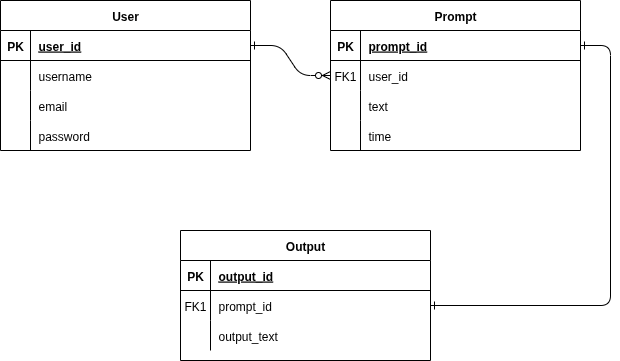
\includegraphics[width=1\textwidth]{images/er_diagram.png}
  \caption{Entity-Relationship Diagram of FormalNet}
  \label{fig:er}
\end{figure}
The Entity Relationship Diagram represents the data model of the FormalNet system. It defines the structure of the database and the relationships between various entities.

In the FormalNet system:
\begin{itemize}
    \item A User can submit multiple Prompts, forming a one-to-many relationship.
    \item Each Prompt is processed by the model, and the corresponding FormalOutput is generated and stored, establishing a one-to-one relationship between Prompt and Output.
    \item Foreign keys maintain referential integrity between the tables
\end{itemize}
This diagram helps in designing an efficient database schema and serves as a foundation for backend development and query optimization.


\section{Dataflow Diagram}
\begin{figure}[H]
  \centering
  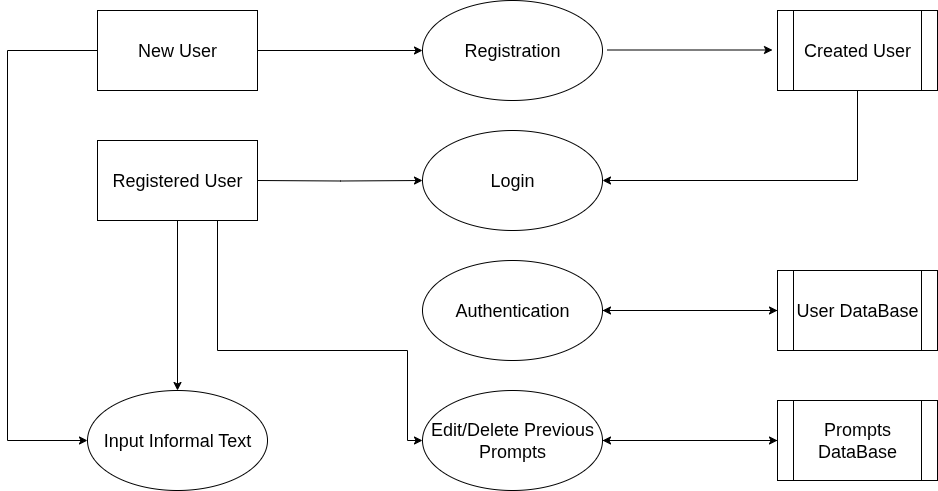
\includegraphics[width=1\textwidth]{images/dataflowdiagram.png}
  \caption{Dataflow Diagram of FormalNet}
  \label{fig:df}
\end{figure}
The data flow diagram (DFD) of the FormalNet system illustrates the movement of data between users, processes, and data stores. It shows how new users register and have their information stored, while registered users can log in and be authenticated using the user database. After authentication, users can input informal text for processing or manage their previous prompts. These actions interact with dedicated databases for storing user and prompt data. The diagram ensures a clear overview of how data flows through the system in a structured manner.


\section{State Diagram}
\begin{figure}[H]
  \centering
  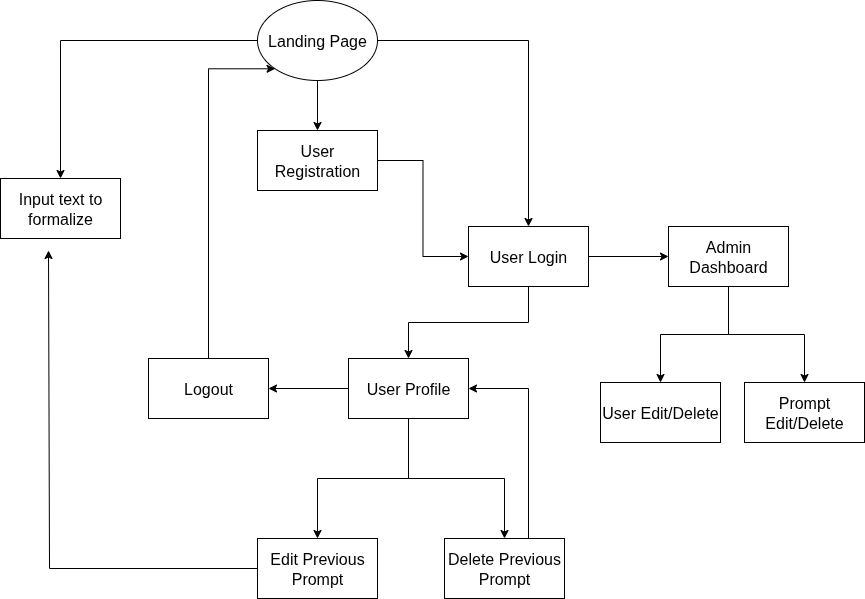
\includegraphics[width=1\textwidth]{images/formalnet state diagram.png}
  \caption{State Diagram of FormalNet}
  \label{fig:statediagram}
\end{figure}
The state diagram of the FormalNet system represents the various states a user or the system can be in during interaction. It begins from the initial state where the user accesses the platform, followed by transitions through states like registration, login, authentication, and text input. Depending on user actions, the system can move to states such as prompt editing or logout. This diagram helps visualize the dynamic behavior of the system and how it responds to different user inputs and transitions.


\section{Use Case Diagram}
\begin{figure}[H]
  \centering
  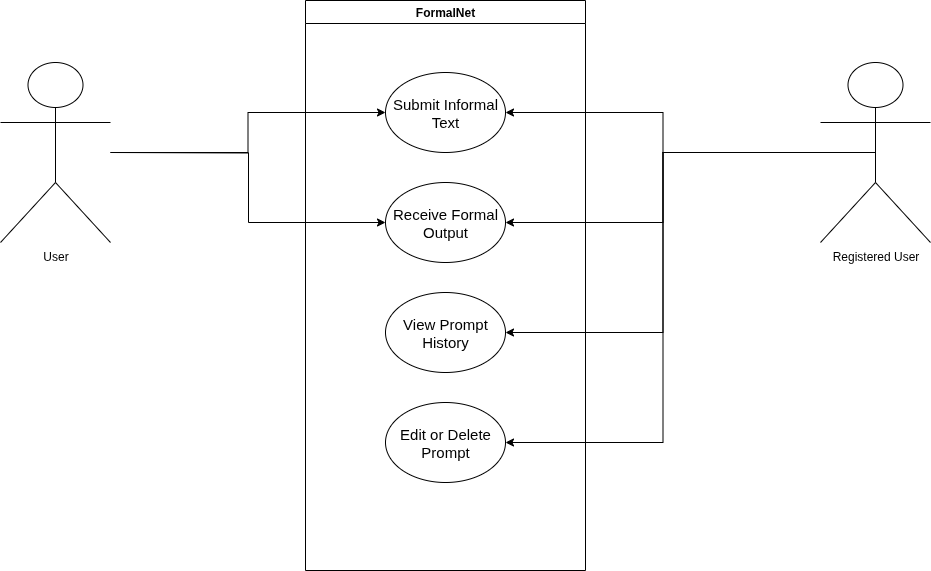
\includegraphics[width=1\textwidth]{images/usecasediagram.png}
  \caption{Use Case Diagram of FormalNet}
  \label{fig:usecase}
\end{figure}
The use case diagram provides a high-level visual representation of the interactions between users (actors) and the system (FormalNet). It outlines the core functionalities that the system offers and the roles that interact with them. This helps in identifying system boundaries and user goals in a clear and concise manner.

There are two main actors in the system:
\begin{itemize}
    \item \textbf{New User}: A user who accesses the system without registration.
    \item \textbf{Registered User}: A user who has an account and can access extended functionalities.
\end{itemize}
The primary use cases shown in the diagram include:
\begin{itemize}
    \item \textbf{Submit Informal Text}: Allows users to input informal text into the system.
    \item \textbf{Receive Formal Output}: The system processes the input and returns a formal version of the text.
    \item \textbf{View Prompt History}: Registered users can view their previous inputs and outputs.
    \item \textbf{Edit or Delete Prompt}: Enables users to manage their past prompts for corrections or updates.
\end{itemize}
This diagram helps in understanding the user interaction flow and serves as a blueprint for system behavior from the user's perspective.

\section{Model Architecture}
\begin{figure}[H]
  \centering
  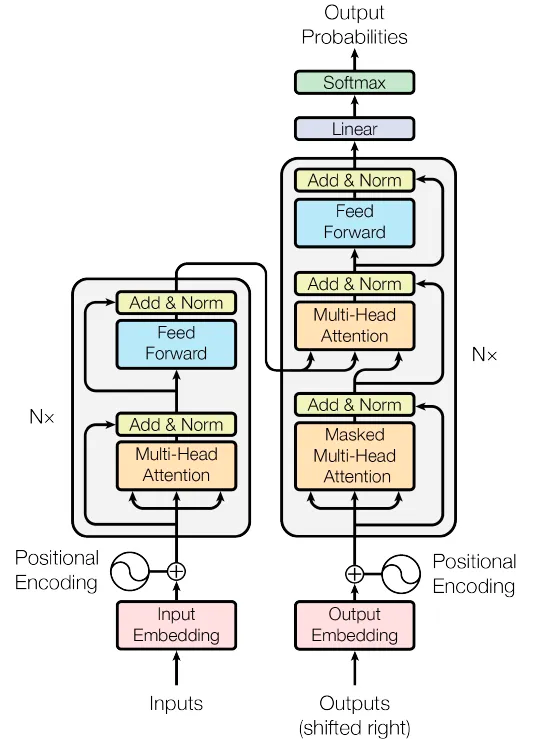
\includegraphics[width=1\textwidth]{images/transformer_architecture.png}
  \caption{Transformer Architecture}
  \label{fig:transformer}
\end{figure}
FormalNet uses a T5 (Text-to-Text Transfer Transformer) model as its core engine for converting informal sentences into formal ones. T5 treats every NLP task as a text generation problem, making it suitable for style transfer tasks.

The model follows the typical encoder-decoder architecture:
\begin{itemize}
  \item \textbf{Encoder:} Encodes the informal input sentence into a latent representation using self-attention.
  \item \textbf{Decoder:} Generates the formal version of the sentence, attending to the encoded input at each step.
\end{itemize}

We used the \texttt{t5-base} variant, which consists of:
\begin{itemize}
  \item 12 Transformer layers each for encoder and decoder
  \item 768-dimensional hidden layers
  \item 12 attention heads
  \item ~220 million parameters
\end{itemize}

The T5 model was fine-tuned on a NUS Social Media Corpus\cite{NUS_Dataset} containing informal and formal sentence pairs. The training pipeline included:

\begin{itemize}
  \item \textbf{Data preprocessing:} Text normalization, tokenization using T5 tokenizer, and input formatting.
  \item \textbf{Model loading:} Initialized from \texttt{t5-base} pretrained weights.
  \item \textbf{Training loop:} Used AdamW optimizer, and early stopping to prevent overfitting.
  \item \textbf{Evaluation:} Model was evaluated using BLEU score and manual quality inspection.
\end{itemize}
Training was performed using PyTorch on a P100 GPU provided by Kaggle.
\newpage


\bibliographystyle{IEEEtran}
\bibliography{references}
\end{document}
